\documentclass[12pt, titlepage]{article}
\usepackage{graphicx}
\usepackage{anysize}
\usepackage{dsfont}
\usepackage{fullpage}
\usepackage{verbatim}
\usepackage{url}
\usepackage{dsfont}
\usepackage[titletoc]{appendix}
\usepackage{tocloft}
\usepackage{url,amsfonts, amssymb, amsthm,color, enumerate, multicol}
\usepackage{amsmath}
\usepackage{placeins}
\usepackage{titlesec}
\usepackage{csvsimple, longtable, booktabs, makecell,siunitx}
\usepackage{subcaption}

\usepackage{mathtools}

\renewcommand{\thesection}{\Roman{section}}
\renewcommand{\thesubsection}{\thesection.\Roman{subsection}}

%\titleformat*{\section}{\normalfont\bfseries}

% Ceil and Floor
\DeclarePairedDelimiter{\ceil}{\lceil}{\rceil}
\DeclarePairedDelimiter\floor{\lfloor}{\rfloor}
%\noprintanswers

\setlength{\cftsecnumwidth}{4em}

\begin{document}

\title{\LARGE \textbf{Police Shootings in the United States} \\
	\vspace{2ex}
	\large VE401 Probabilistic Methods in Engineering \\
    Project 2 (Summer 2017)}
\date{June 23, 2017}
\author{\textit{Siddharth Ramesh}\\ \textit{Ziwen Lu}\\ \textit{Kevin Zheng}\\ \textit{Derek Tan}\\ \textit{Chengcheng Zhu}}

\maketitle



\pagenumbering{gobble}
\pagebreak
\tableofcontents
\pagebreak
\setcounter{page}{1}
\pagenumbering{arabic}

\section{Introduction}

In 2016, the Washington Post \cite{washington} released an article regarding police homicides in the USA. Since Jan 1, 2015, the Post has been maintaining a detailed database of each shooting that takes place, including particulars such as the race and gender of the deceased, the circumstances of the situation and the manner of defense used by the deceased in the situation. This project examines this database from a statistical point of view, based on the article \textit{London murders: a predictable pattern?} by David Spiegelhalter and Arthur Barnett \cite{barnett}.\\
The Washington Post uses a variety of sources to keep its database on police shootings up to date. These include local news and social media reports, law enforcement websites, and independent sources (such as the database known as 'Killed by Police and Fatal Encounters'). In order to make their information as accurate as possible, the Post cross-confirms their data with other sources such as the FBI and the CDC and maintains an open email for information regarding police homicides. The term 'fatal police shooting' or 'police homicide' here specifically refers to a situation in which a police officer shoots and kills a civilian in the line of duty. Deaths caused by police officers that are off duty, by any method apart from a shooting or those that occur during police custody are not considered.

\section{Police Homicides - 2015 through 2016}

\begin{figure}[h]
\centering
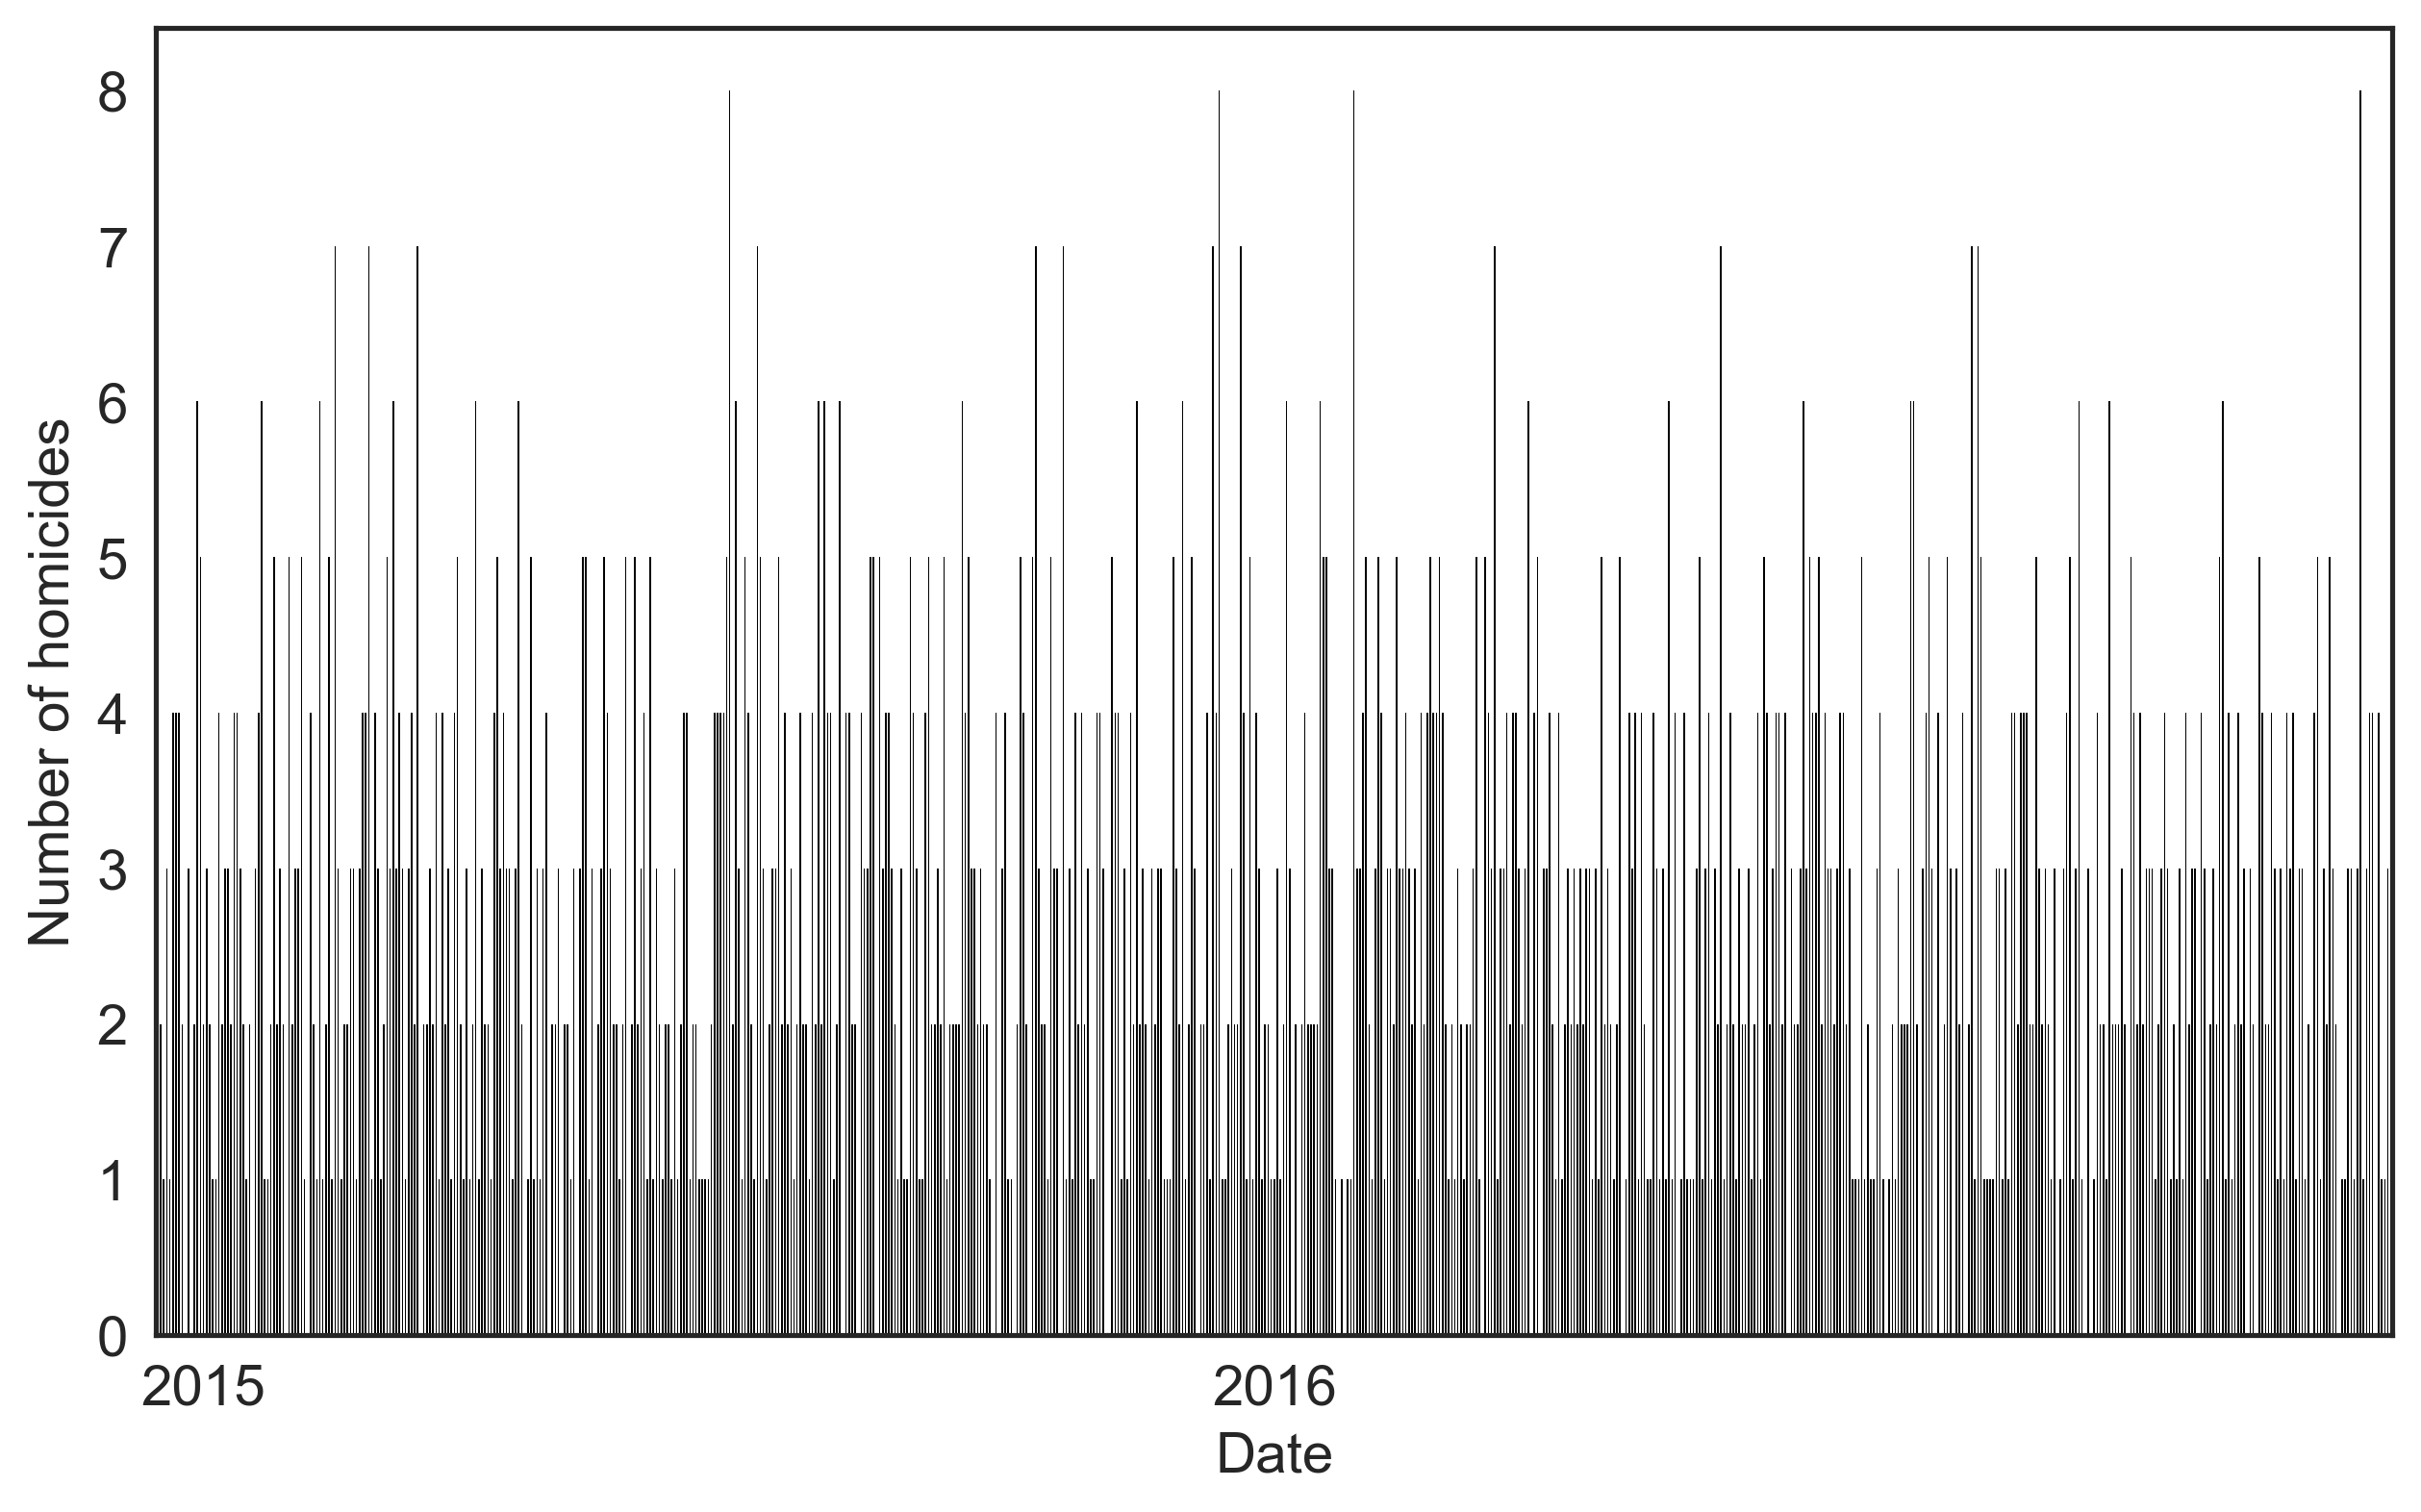
\includegraphics[width=\textwidth]{assets/homicides_frequency_(ii).png}
\caption{Homicides Per Day 2015 through 2016\cite{washington}}
\end{figure}

\subsection{Frequency of Shootings}

During the period of January 2015 through December 2016, there have been 1954 homicides over 731 days in the United States recorded by the Washington Post \cite{washington}. There were only 50 days without a police homicide. Figure 1 visualizes these police homicides per day over this two year period.\\
It is important to note that 2016 is a leap year, so February has an extra day. We have decided to simply include the extra day as is with the data, keeping in mind to adjust for the number of days, weekdays, and number of days for February.

\subsection{Goodness-of-fit test for Poisson Distribution}
Spiegelhalter and Barnett \cite{barnett} found that the London murders followed a Poisson distribution with parameter k = 0.44. We would like to see if police homicides in the United States also fit a Poisson distribution. To begin, we need to find an estimate for the unknown parameter k. We know that the maximum likelihood estimator for k is \^{k} = $\bar{X}$, so from the data in Table 1, \^{k} = 2.673.
\begin{proof}
\begin{equation}
\begin{split}
L(k) & = \prod_{i = 1}^{n}\frac{e^{-k}k^{x_i}}{x!} \\
& = \frac{e^{-nk}k^{\sum x_i}}{\prod x!}\\
ln(L(k)) & = -nk + ln(k)\sum x_i - ln(\prod x!) \\
\frac{d}{dk} ln(L(k)) & = -n + \frac{\sum x_i}{k} = 0 \\
\therefore \hat{k} & = \frac{1}{n}\sum x_i = \bar{X}
\end{split}
\end{equation}
\end{proof}
\csvreader[
  longtable=cccc,
  table head=
  \toprule \bfseries \thead{X} & \bfseries \thead{Observed} & \bfseries \thead{Expected} & \bfseries \thead{Probability}\\\midrule\endhead,
  late after line=\\,
  before reading={\catcode`\#=12},after reading={\catcode`\#=6},
  table foot = \bottomrule \caption{Observed and expected frequencies of days with X number of police homicides using 2015-2016 data corresponding to a Poisson distribution with parameter k = 2.673}
]{assets/poisson_15_16.csv}{1=\one, 2=\two, 3=\three, 4=\four}{\one & \two & \three & \four}

\pagebreak

\noindent Our claim is \\
$H_0$: Police homicides per day follows a Poisson distribution with parameter k = 2.673 \\
which is equivalent to \\
$H_0$: Police homicides per day follows a Multinomial distribution with parameters (.069, .185, 0.247, 0.220, 0.147, 0.079, 0.035, 0.013, 0.006)\\

\noindent For n = 9 categories, one parameter estimated, the statistic follows a $\chi^2$ distribution with 9 - 1 - 1 = 7 degrees of freedom.
\begin{equation}
\begin{split}
	\chi^2 & = \sum_{i = 1}^n \frac{(O - E)^2}{E} = 4.84 \\
	\chi^2_{7, .05} & = 14.07
\end{split}
\end{equation}
Since 4.84 $\ngtr$ 14.07, we fail to reject $H_0$ at significance 0.05; there is no evidence that the data does not follow a Poisson distribution.\\
Using this Poisson distribution with parameter k = 2.673, we can examine the predicted number of homicides, shown in Figure 2.
\begin{figure}[ht!]
    \centering
    \begin{subfigure}[t]{0.5\textwidth}
        \centering
        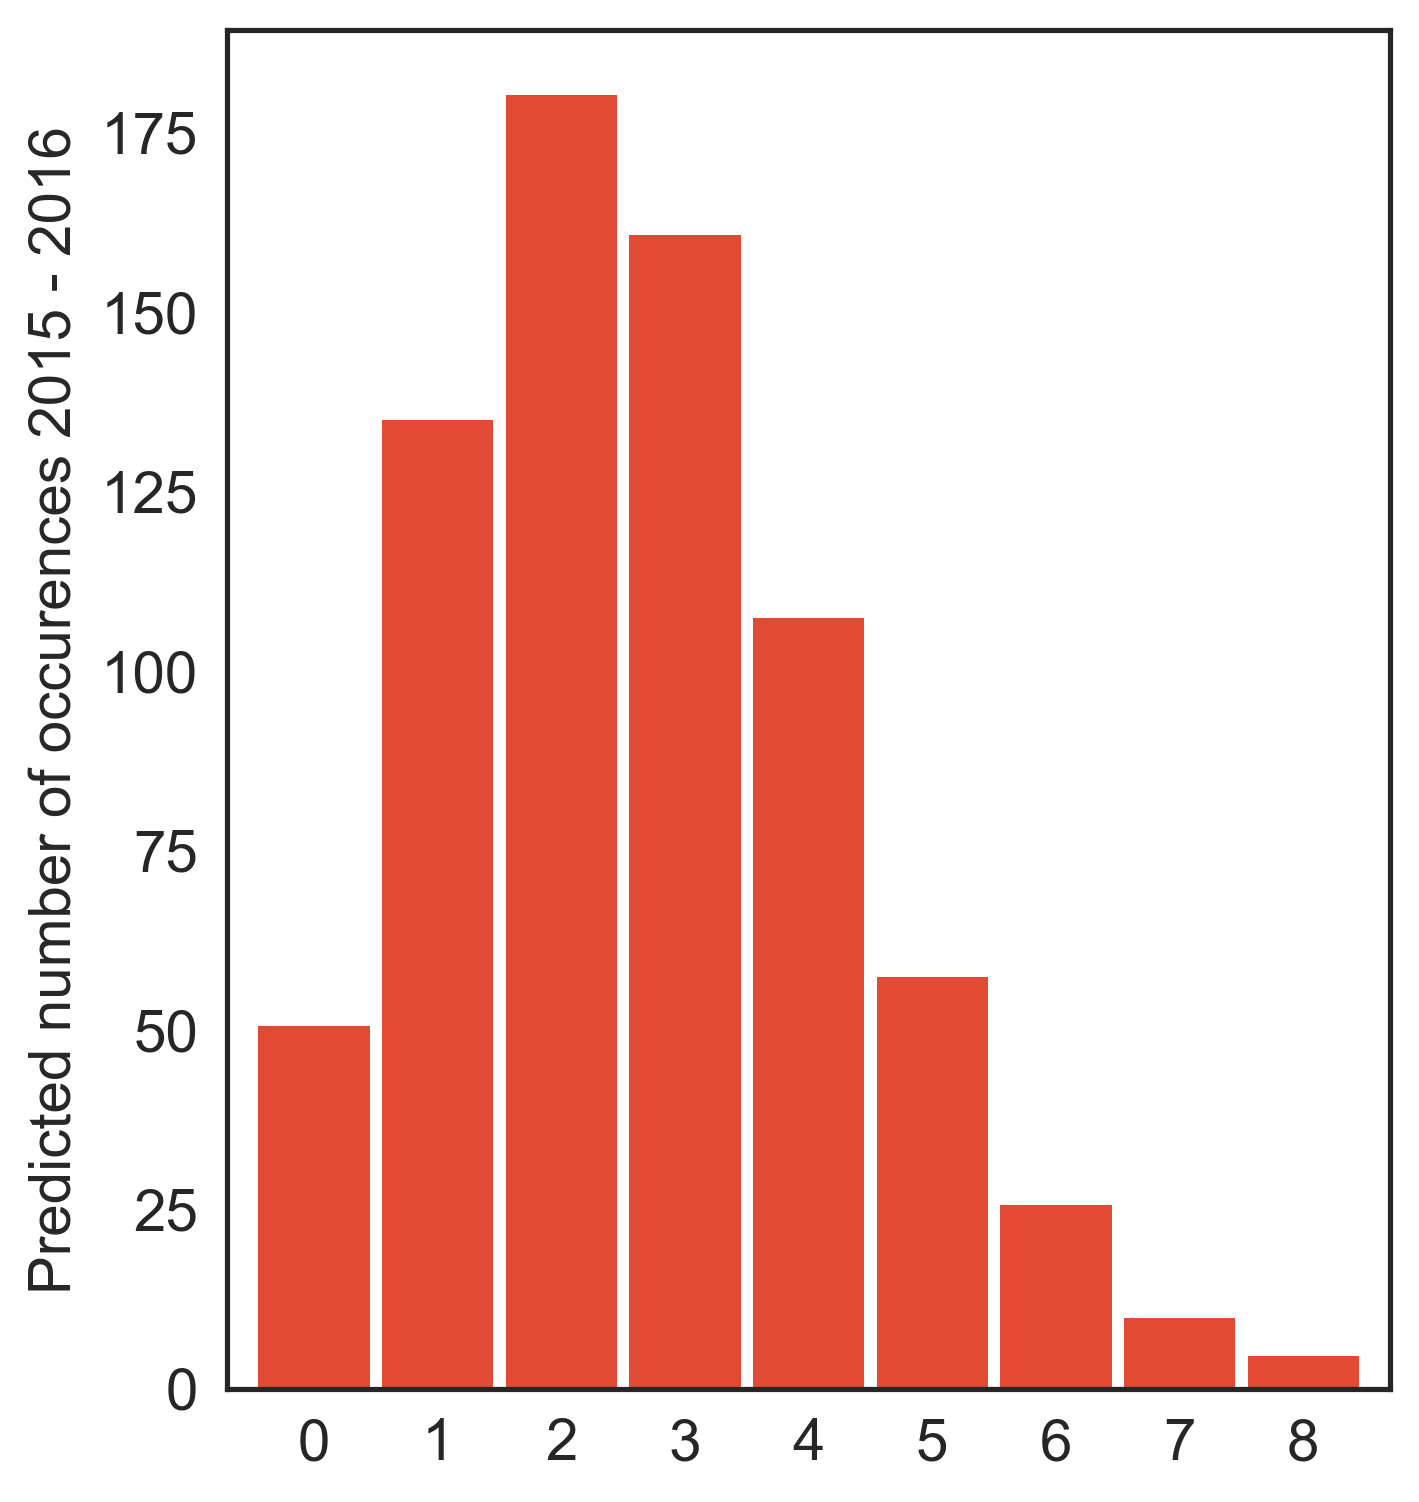
\includegraphics[width=.9\textwidth]{assets/day_frequency_poisson_(iiia).png}
        \caption{Homicides Per Day}
    \end{subfigure}%
    ~ 
    \begin{subfigure}[t]{0.5\textwidth}
        \centering
        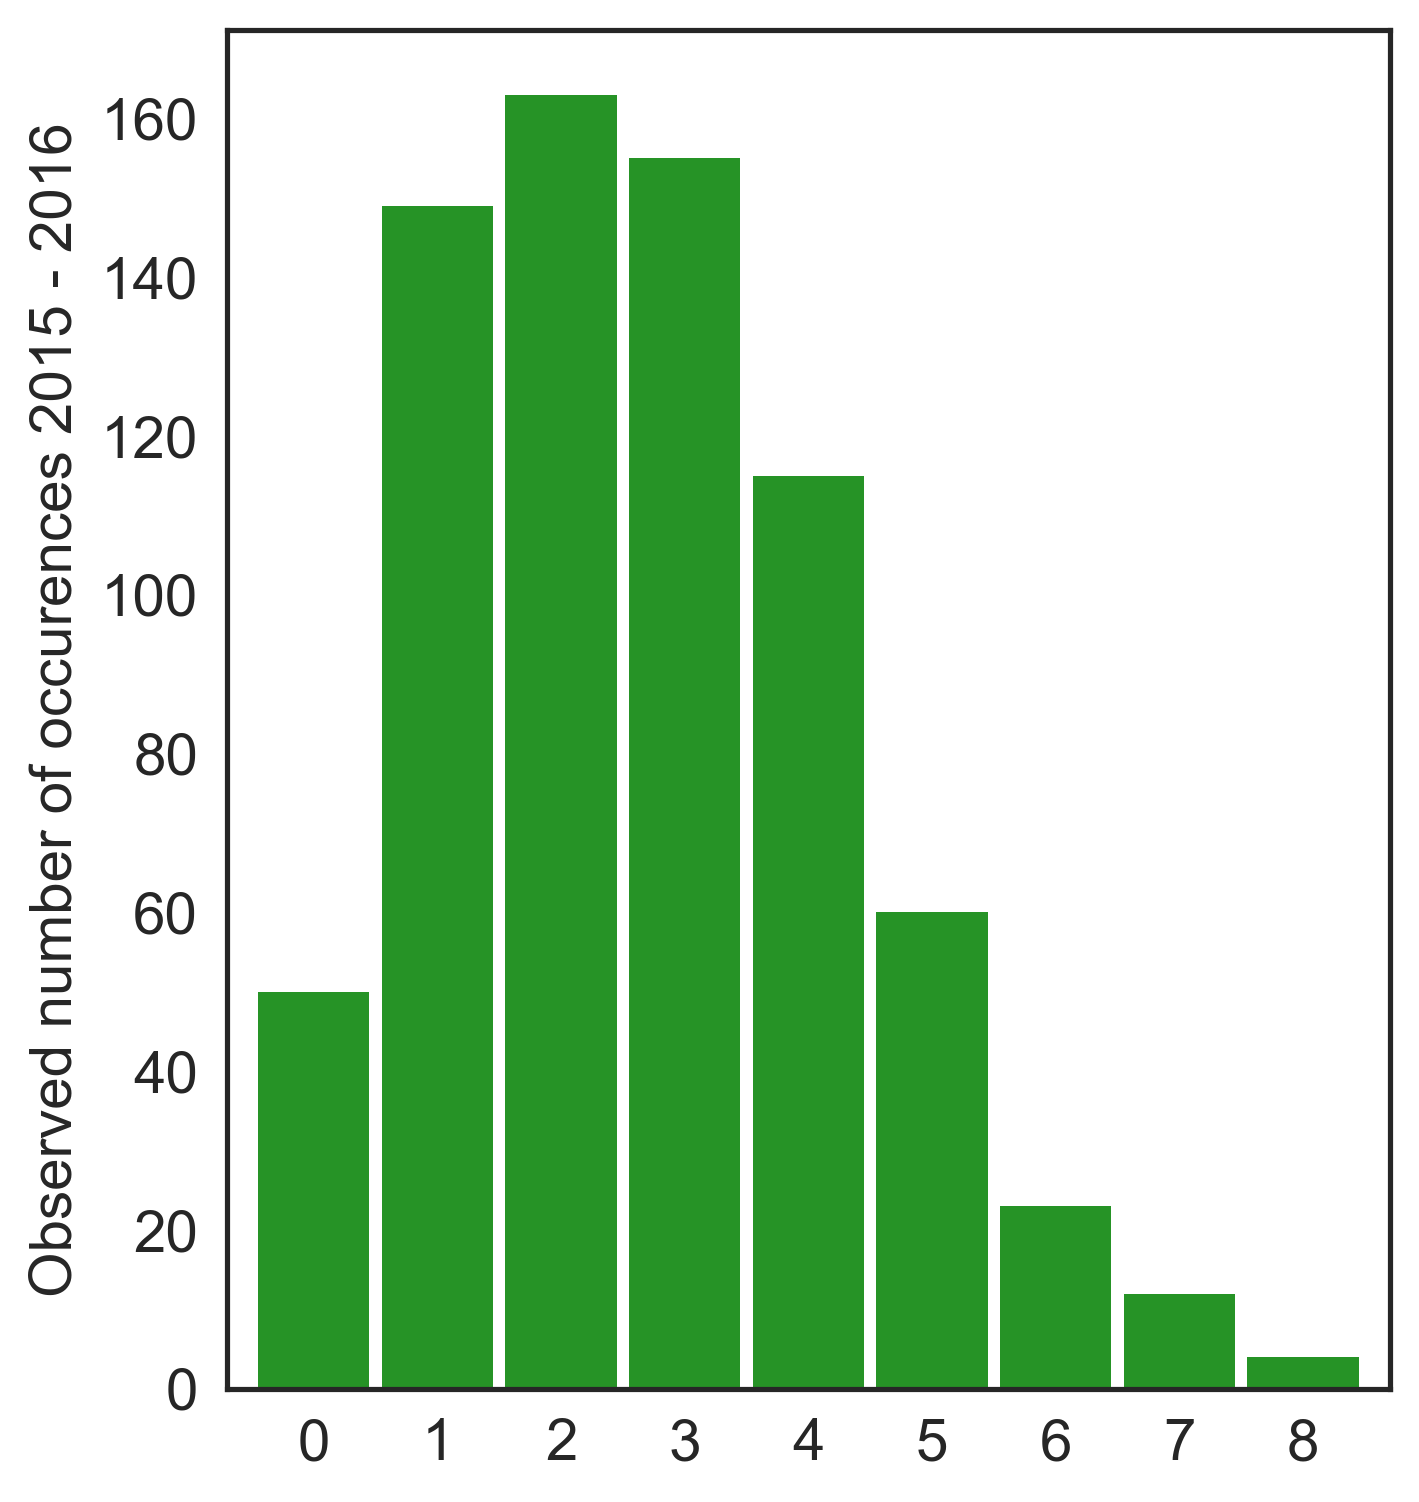
\includegraphics[width=.9\textwidth]{assets/day_frequency_poisson_(iiib).png}
        \caption{Homicides Per Day}
    \end{subfigure}
    \caption{Predicted and observed frequencies of days with different numbers of Police Homicides between January 2015 through December 2016; (a) predicted, (b) observed}
\end{figure}

From the data, it seems that the Poisson distribution models the observed occurences well, with 2 or 3 homicides in a single day being the most likely. To help shed light on this, we can analyze the homicides deeper through Table 2 by looking at the methods of aggravation. Note that the majority of police homicides (55\%) have been aggravated by a gun. With 1074 police homicides aggravated by guns alone, it may seem less ridiculous that there are so many expected (and actual) shootings per day.
\pagebreak

\csvreader[
  longtable=cccc,
  table head=
  \toprule \bfseries \thead{Method of \\Aggravation} & \bfseries \thead{Rank} & \bfseries \thead{Frequency} & \bfseries \thead{Percentile (\%)}\\\midrule\endhead,
  late after line=\\,
  before reading={\catcode`\#=12},after reading={\catcode`\#=6},
  table foot = \bottomrule \caption{Most common methods of aggravation leading to a Police Homicide; other weapons were grouped into a category of frequency less than 10}
]{assets/weapons.csv}{1=\one, 2=\two, 3=\three, 4=\four}{\one & \two & \three & \four}

\subsection{Police Homicides by Week and Month}

\begin{figure*}[ht!]
    \centering  
    \begin{subfigure}[t]{0.5\textwidth}
        \centering
        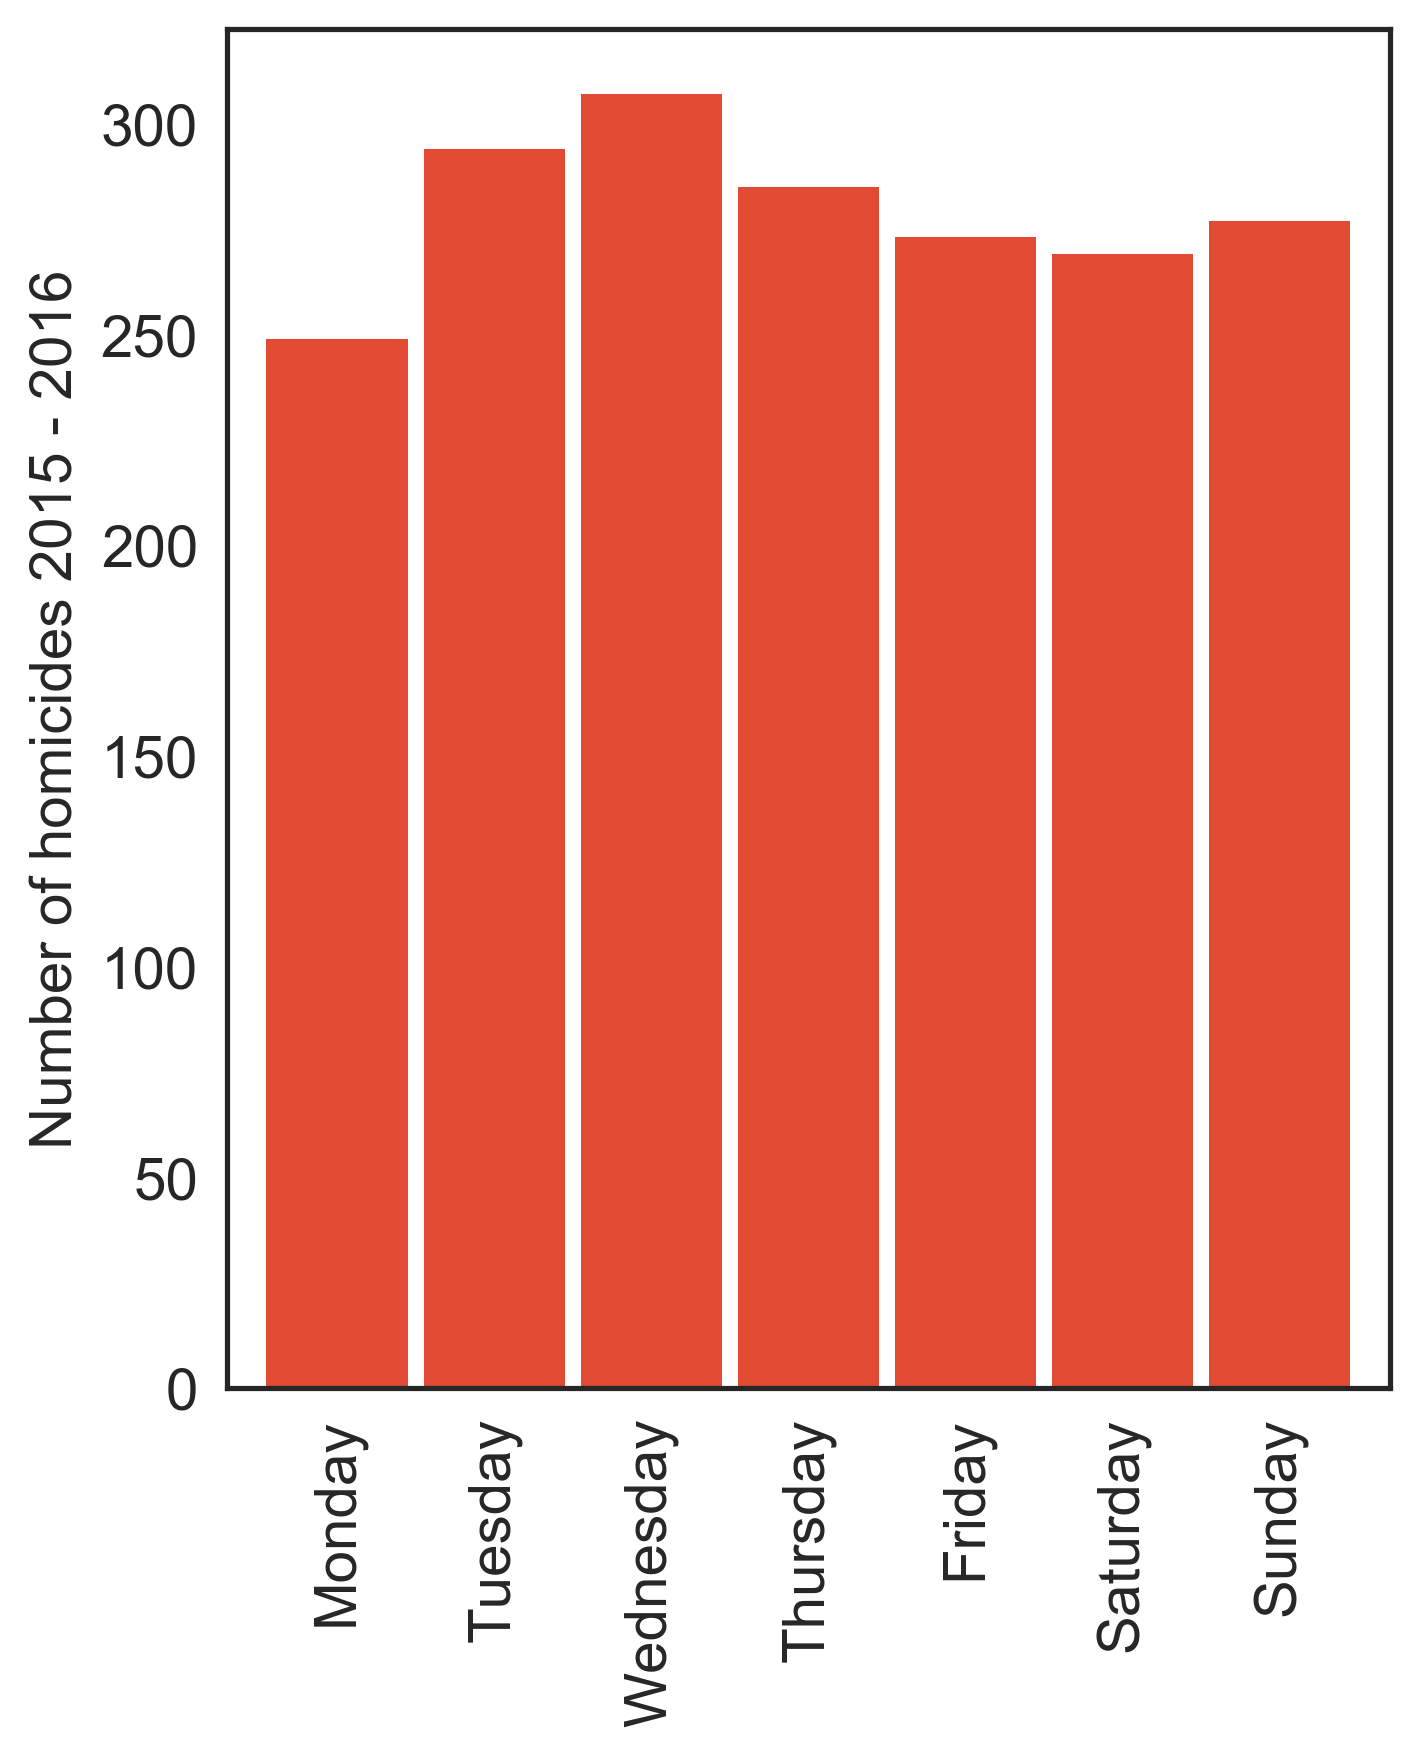
\includegraphics[width=.9\textwidth]{assets/week_month_frequency_(iva).png}
        \caption{Homicides by Weekday}
    \end{subfigure}%
    ~ 
    \begin{subfigure}[t]{0.5\textwidth}
        \centering
        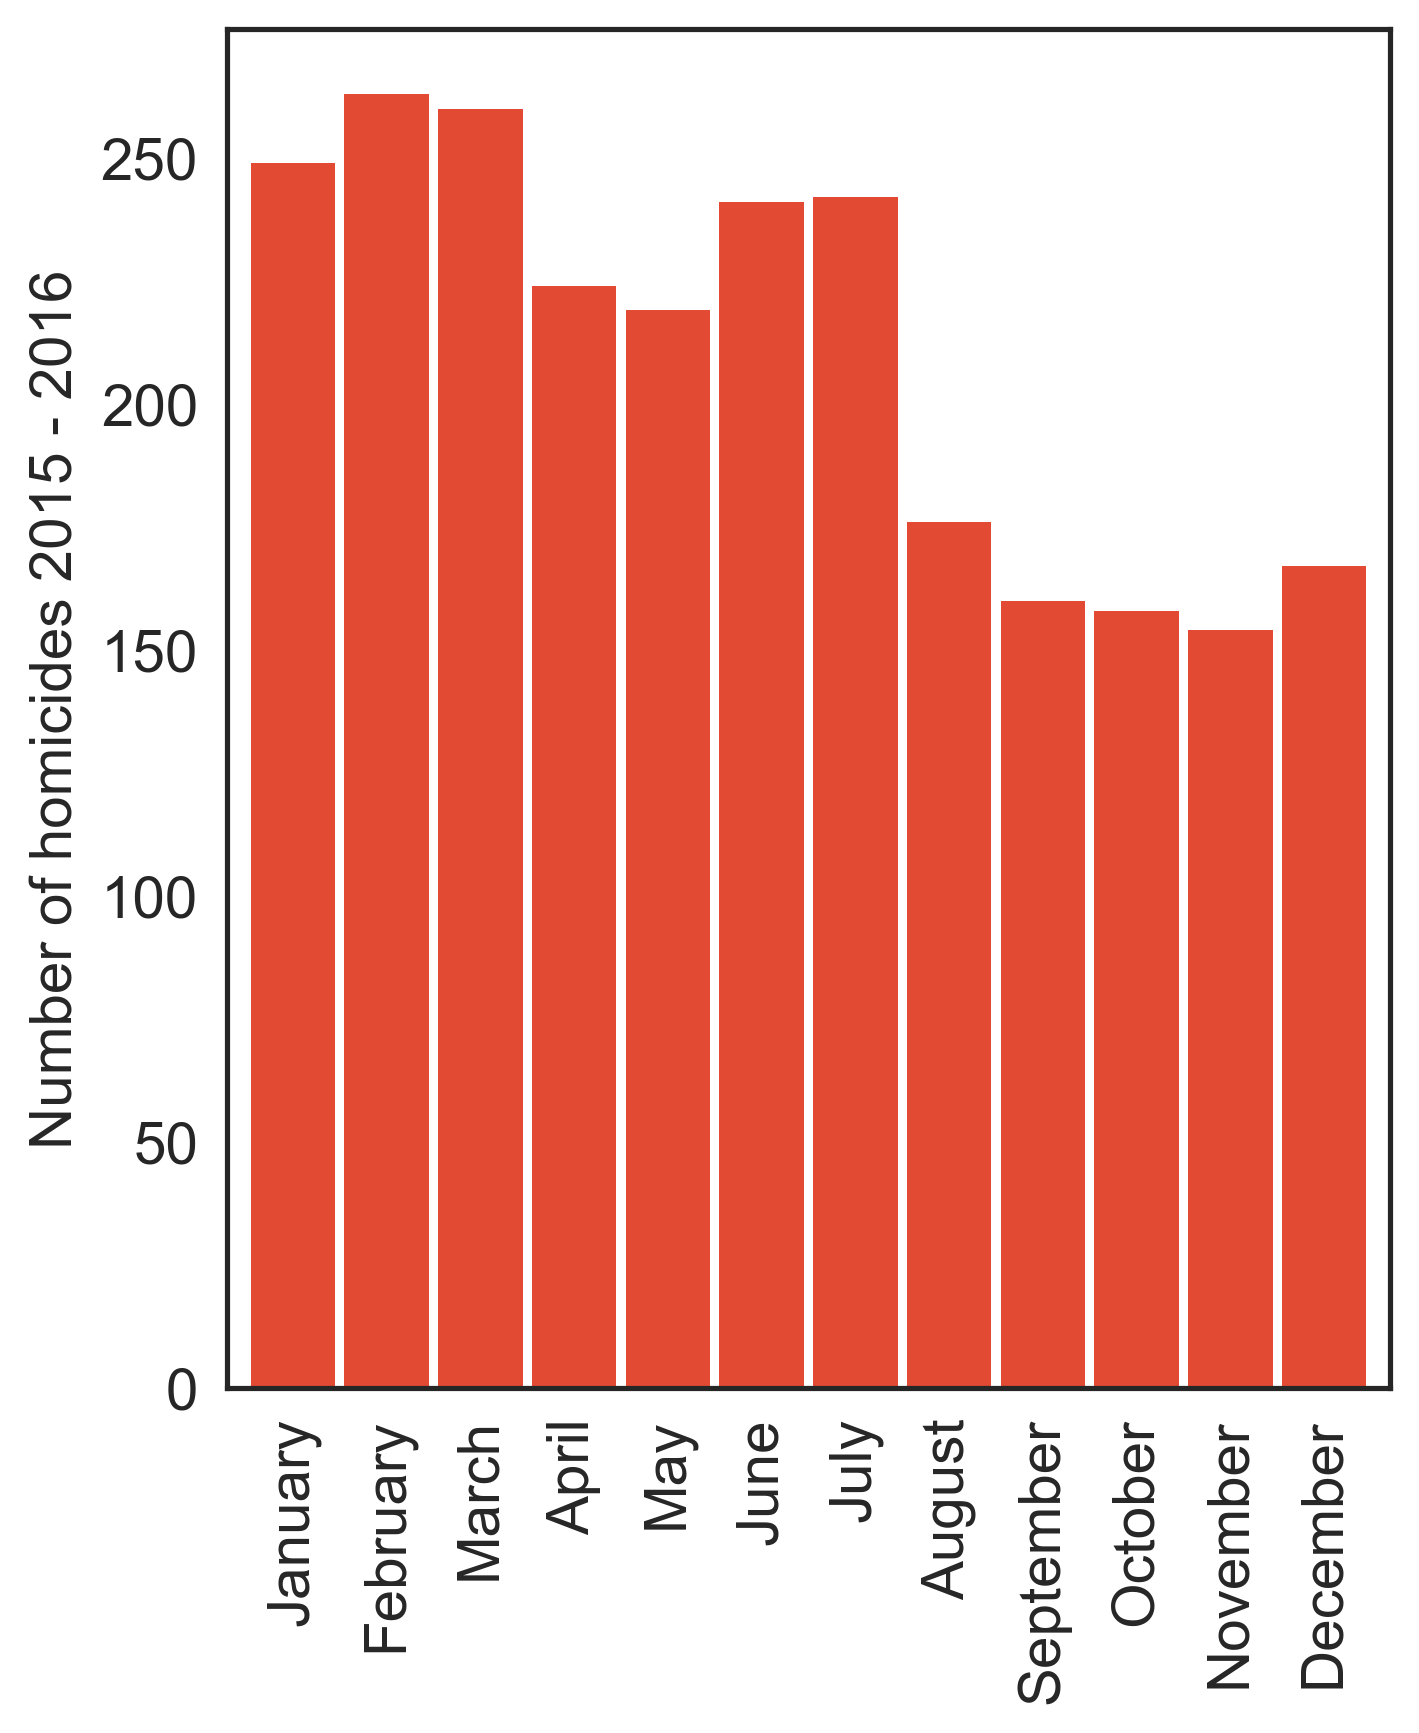
\includegraphics[width=.9\textwidth]{assets/week_month_frequency_(ivb).png}
        \caption{Homicides by Month}
    \end{subfigure}
	\caption{Total Police Homicides by weekday and month between January 2015 through December 2016; (a) weekday, (b) monthly}
\end{figure*}

\setcounter{table}{0}

\begin{table}[ht!]
    \centering
    \begin{subtable}[t]{0.5\textwidth}
		\csvreader[
		longtable=cccc,
		no head,
		table head=
		\toprule \bfseries \thead{Month} & \bfseries \thead{Frequency}\\\midrule\endhead,
		late after line=\\,
		table foot = \bottomrule
		]{assets/wk_freq.csv}{1=\one, 2=\two}{\one & \two}
		\caption{Police Homicides by weekday}
    \end{subtable}%
    \begin{subtable}[t]{0.5\textwidth}
		\csvreader[
		longtable=cccc,
		no head,
		table head=
		\toprule \bfseries \thead{Month} & \bfseries \thead{Frequency}\\\midrule\endhead,
		late after line=\\,
		table foot = \bottomrule
		]{assets/month_freq.csv}{1=\one, 2=\two}{\one & \two}
		\caption{Police Homicides by month}
    \end{subtable}
    \caption{Total Police Homicides by weekday and month between January 2015 through December 2016; (a) weekday, (b) monthly}
\end{table}
\pagebreak
Given the data in Table 3, there seems to be a rise in shootings during the middle of the week; perhaps the number of police shootings depends on the weekday. Is this statistically significant?\\

We have decided to use an ANOVA test with k = 7 populations corresponding to each weekday. We test \\
$H_0: \mu_1 = \mu_2 = \mu_3  = \mu_4 = \mu_5 = \mu_6 = \mu_7$ \\ 
$H_1: \mu_i \neq \mu_j$ for at least one i, j $\in 1 \leq i \leq j \leq 7$ \\
$\mu_i$ corresponds to the ith day of the week (starting on Monday) \\

Applying this test gives us the following ANOVA table:
\csvreader[
  longtable=ccccc,
  table head=
  \toprule \bfseries \thead{Source of\\Variation} & \bfseries \thead{Degrees of\\Freedom} & \bfseries \thead{Sum of\\Squares} & \bfseries \thead{Mean Square} & \bfseries \thead{F-value}\\\midrule\endhead,
  late after line=\\,
  before reading={\catcode`\#=12},after reading={\catcode`\#=6},
  table foot = \bottomrule
]{assets/anova.csv}{1=\one, 2=\two, 3=\three, 4=\four, 5=\five}{\one & \two & \three & \four & \five}
with a p-value of 0.27. Thus, with such a high p-value, we have insufficient evidence to reject $H_0$; there does not seem to be a dependency of police homicides on the weekday.

\pagebreak

\subsection{Confidence Intervals for Poisson parameter}
Since the estimator for k is dependent on our data and may change as time goes on, we are interested in finding a confidence interval. By the central limit theorem, since we have a large sample size, we assume that $\hat{k} = \bar{X}$ follows an approximate normal distribution with mean $k$ and variance $\frac{k}{n}$. \\

\begin{proof}
\begin{equation*}
\begin{split}
E[\hat{k}] & = E[\bar{X}] = E[\frac{1}{n}\sum_{i=1}^n x_i] = \frac{1}{n} \sum_{i=1}^n E[x_i] \\
& = \frac{1}{n} \sum_{i=1}^n k \hspace{5ex} \text{as $x_i$ follows a Poisson distribution}\\
& = \frac{1}{n} nk = k  
\end{split}
\end{equation*}
\end{proof}

\noindent Then with our normal assumption, the Poisson parameter is modeled by
\begin{equation*}
Z = \frac{\hat{k} - k}{\sqrt{k/n}}
\end{equation*}
with a confidence interval
\begin{equation*}
\hat{k} \pm z_{\alpha/2}\sqrt{k/n} 
\end{equation*}
\noindent In practice, k is an unknown parameter that we are trying to estimate in the first place. To work around this, we can substitute the $\sqrt{k/n}$ with $\sqrt{\hat{k}/n}$, which is valid under the assumption that \^{k} is approximately normally distributed.\\

Using the data in Table 1, we have $\hat{k} = 2.673$ and n = 731. For a 95\% confidence interval, we set our $\alpha = 0.05$.
\begin{equation*}
k = \hat{k} \pm z_{\alpha/2}\sqrt{\hat{k}/n} = 2.673 \pm 1.96\sqrt{2.673/731} = 2.673 \pm 0.119 = [2.554, 2.792]
\end{equation*} 

\pagebreak

\section{Police Shootings 2017 - Present}

\subsection{Goodness-of-fit test for Poisson Distribution}
Using data from 2017 to the present (June 23, 2017), we can perform the hypothesis test again to see if the data follows a Poisson distribution. We can also see if the estimated parameter k is within the confidence interval found in the previous section.\\

\noindent From the data in Table 4, $\hat{k} = \bar{X}$ = 2.740

\csvreader[
  longtable=cccc,
  table head=
  \toprule \bfseries \thead{X} & \bfseries \thead{Observed} & \bfseries \thead{Expected} & \bfseries \thead{Probability}\\\midrule\endhead,
  late after line=\\,
  before reading={\catcode`\#=12},after reading={\catcode`\#=6},
  table foot = \bottomrule \caption{Observed and expected frequencies of days with X number of police homicides using 2017 data corresponding to a Poisson distribution with parameter k = 2.740}
]{assets/poisson_17_a.csv}{1=\one, 2=\two, 3=\three, 4=\four}{\one & \two & \three & \four}

We cannot use the Pearson statistic to test that the data fits a Poisson distribution because more than 20\% of our categories have an expected value less than 5. We merge the last two rows to fit this constraint.

\csvreader[
  longtable=cccc,
  table head=
  \toprule \bfseries \thead{X} & \bfseries \thead{Observed} & \bfseries \thead{Expected} & \bfseries \thead{Probability}\\\midrule\endhead,
  late after line=\\,
  before reading={\catcode`\#=12},after reading={\catcode`\#=6},
  table foot = \bottomrule \caption{Observed and expected frequencies of days with X number of police homicides using 2017 data corresponding to a Poisson distribution with parameter k = 2.740}
]{assets/poisson_17_b.csv}{1=\one, 2=\two, 3=\three, 4=\four}{\one & \two & \three & \four}
\pagebreak
\noindent Then we test \\
$H_0$: Data follows a Poisson distribution with parameter k = 2.740 \\
which is equivalent to \\
$H_0$: Data follows a Multinomial distribution with parameters (0.065, 0.177, 0.242, 0.221, 0.152, 0.083, 0.038, 0.022)

\noindent For n = 8 categories, with one parameter estimated, the statistic follows a $\chi^2$ distribution with 8 - 1 - 1 = 6 degrees of freedom.
\begin{equation*}
\begin{split}
  \chi^2 & = \sum_{i = 1}^n \frac{(O - E)^2}{E} = 2.11 \\
  \chi^2_{6, .05} & = 12.59
\end{split}
\end{equation*}
Since 2.11 $\ngtr$ 12.59, we fail to reject $H_0$ at significance 0.05; there is insufficient evidence to say that the data does not follow a Poisson distribution.\\

\noindent Then, we can also see that $2.740 \in [2.554, 2.792]$, the confidence interval for the 2015-2016 data that we found earlier, which further validates that the data fits a Poisson distribution.

\subsection{Prediction Intervals}
\subsubsection{Nelson's formula}
Now, we wish to find an interval that predicts where a new, unknown value will likely fall. We use the Nelson Prediction Interval\cite{Nelson}, where we let X be the total occurences in a sample size of n from a Poisson distribution with mean k and Y be the (predicted) counts from the same Poisson distribution. Thus, $X \sim$ Poisson(nk), $Y \sim$ Poisson(mk). Since we are under the assumption that Y and \^{Y} are approximately normally distributed, hence \^{Y} - Y is normally distributed, the 100(1-$\alpha$)\% prediction interval is then as follows: 
\begin{equation}
  Y = \hat{Y} \pm z_{\alpha/2}\sqrt{m\hat{Y}(\frac{1}{m} + \frac{1}{n})} \hspace{5ex} \text{with \^{Y} = } X \frac{m}{n}
\end{equation}

\begin{proof}
We have
\begin{equation*}
\begin{split}
E[\hat{Y} - Y] & = \mu_Y - \mu_Y = 0 \\
Var[\hat{Y} - Y] & = m^2\hat{k}(\frac{1}{n} + \frac{1}{m}) \\
& = m^2 \frac{\hat{Y}}{m}(\frac{1}{n} + \frac{1}{m})\\
& = m\hat{Y}(\frac{1}{n} + \frac{1}{m}) \\
\therefore Z_{\alpha/2} & \sim \frac{\hat{Y} - Y - E[\hat{Y} - Y]}{\sqrt{Var[\hat{Y} - Y]}} \hspace{5pt}\text{Since Y - \^{Y} follows a normal distribution} \\
& = \frac{\hat{Y} - Y}{\sqrt{m\hat{Y}(\frac{1}{n} + \frac{1}{m})}}
\end{split}
\end{equation*}
\end{proof}

We are interested in finding prediction interval for the cumulative police shootings at a given day. In this case, n is the number of days of data previously that we already have, and m is the number of days that we want to predict in the future. \^{Y} depends on X, m, and n. By plugging 2015 and 2016 data in \^{Y}, m, n into Nelson's formula for each day, we obtain the following prediction interval in Figure 4. It can be seen that as the year progresses, the prediction is more uncertain and gradually diverges.

\begin{figure}[h]
\centering
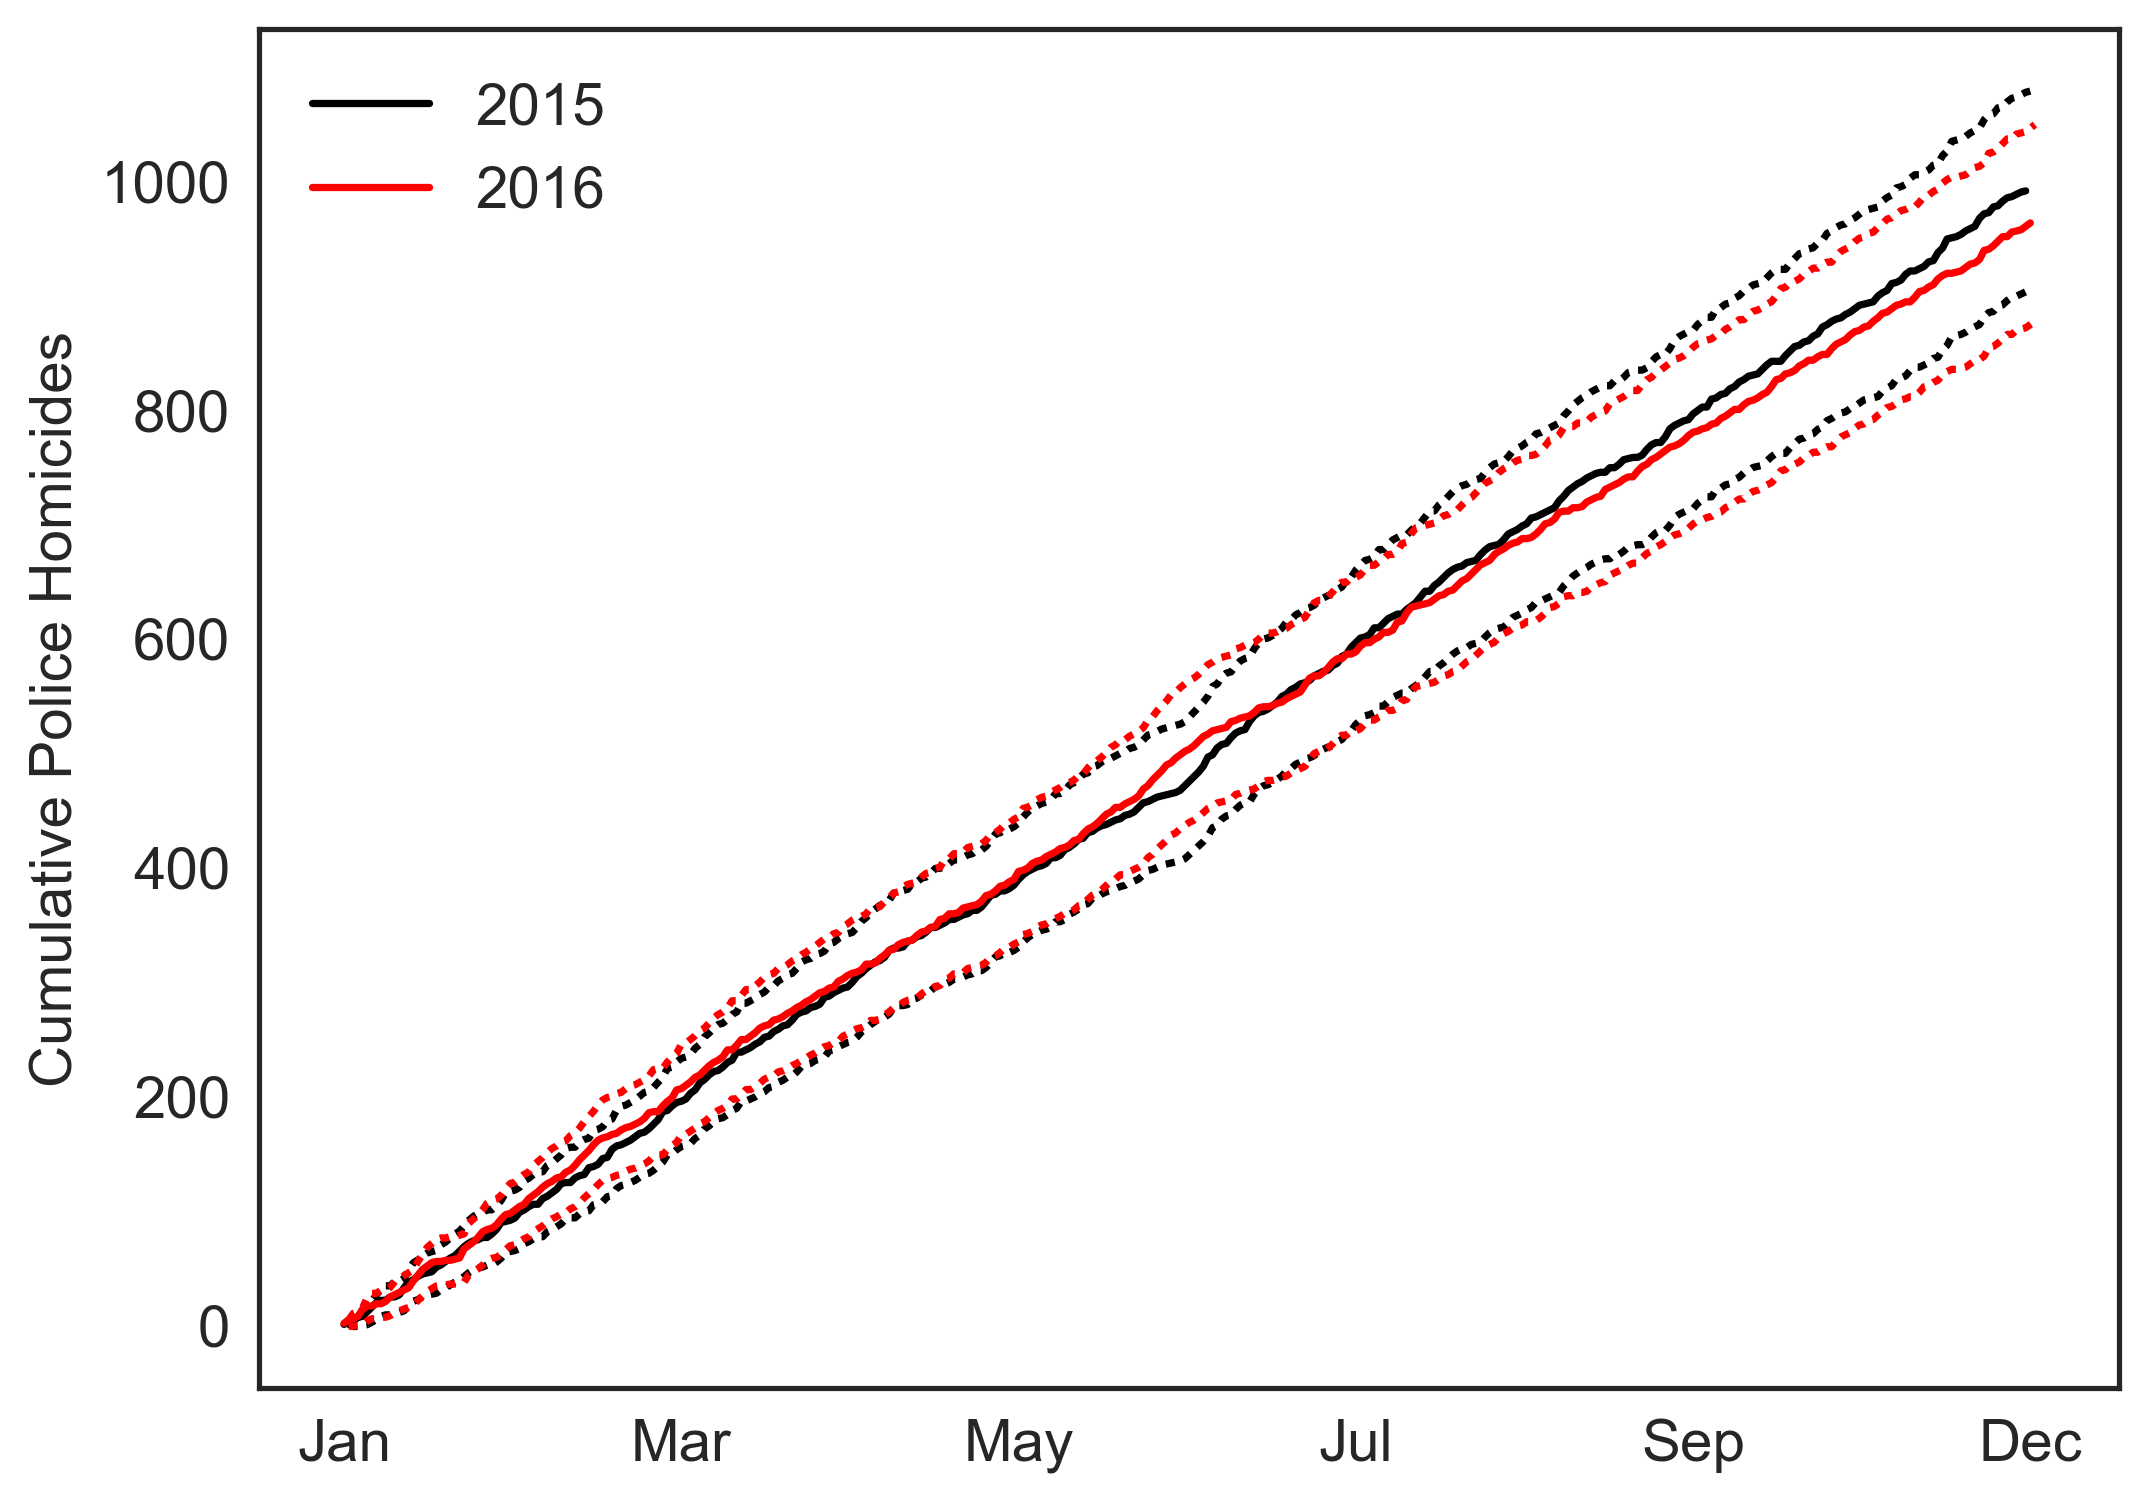
\includegraphics[width=\textwidth*2/3]{assets/cumulative_homicides_(ixa).png}
\caption{Cumulative Police Homicides in 2015 and 2016 with 95\% Prediction Bands\cite{washington}}
\end{figure}

\begin{figure}[h!]
\centering
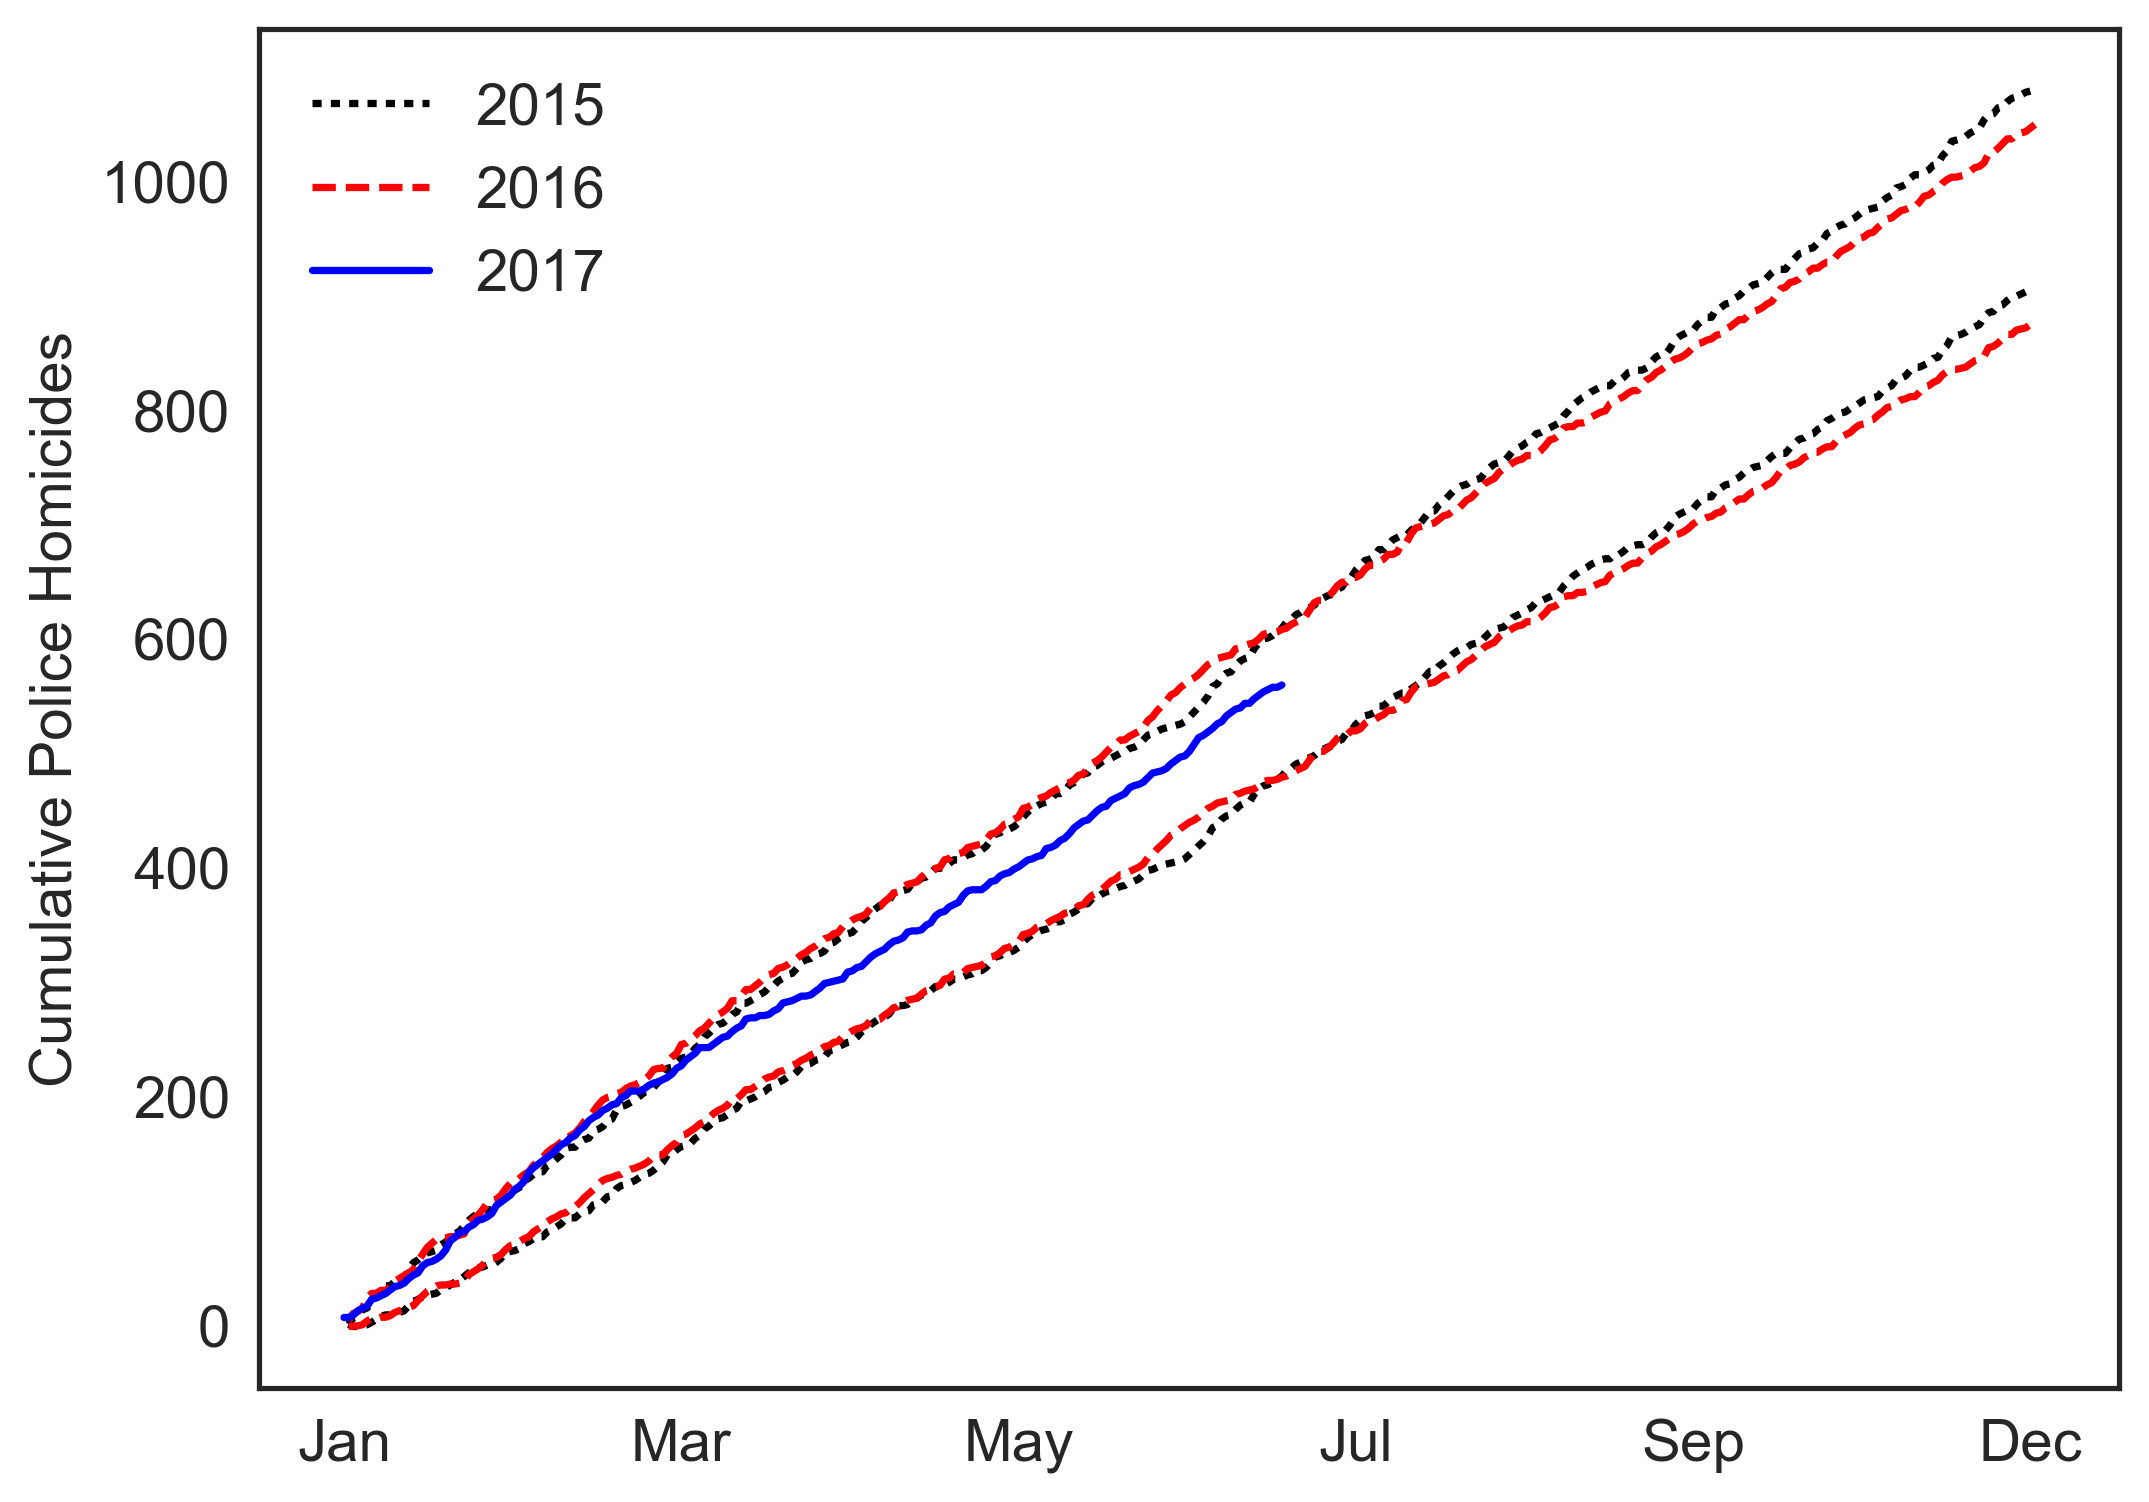
\includegraphics[width=\textwidth*2/3]{assets/cumulative_homicides_(ixb).png}
\caption{Cumulative Police Homicides in 2017 with 95\% Prediction Bands for 2015 and 2016\cite{washington}}
\end{figure}

Is our prediction interval accurate, or does 2017 have an unusually large amount of police shootings? In Figure 5, we overlay the cumulative 2017 police shootings over our prediction bands. We see that towards the beginning of the year in the months from January to March, the police shootings were high but still generally within our 95\% prediction intervals. From March to present, the 2017 data is well within the interval.




\pagebreak

\begin{thebibliography}{9}
\raggedright

\bibitem{Nelson}
K. Krishnamoorthy and Jie Peng. Improved closed-form prediction intervals for binomial and poisson distributions. Journal of Statistical Planning and Inference, 141(5):1709 – 1718, 2011.

\bibitem{washington}
The Washington Post. Fatal force. \url{https://www.washingtonpost.com/graphics/national/ police-shootings-2016/}. Web. Accessed February 16th, 2017.

\bibitem{barnett}
D. Spiegelhalter and A. Barnett. London murders: a predictable pattern? Significance, 6(1):5–8, 2009. \url{http://onlinelibrary.wiley.com/doi/10.1111/j.1740-9713.2009.00334.x/abstract} [Online; accessed 5-July-2015].

\end{thebibliography}




\bibliography{References}

\end{document}
